\PassOptionsToPackage{unicode=true}{hyperref} % options for packages loaded elsewhere
\PassOptionsToPackage{hyphens}{url}
%
\documentclass[]{article}
\usepackage{lmodern}
\usepackage{amssymb,amsmath}
\usepackage{ifxetex,ifluatex}
\usepackage{fixltx2e} % provides \textsubscript
\ifnum 0\ifxetex 1\fi\ifluatex 1\fi=0 % if pdftex
  \usepackage[T1]{fontenc}
  \usepackage[utf8]{inputenc}
  \usepackage{textcomp} % provides euro and other symbols
\else % if luatex or xelatex
  \usepackage{unicode-math}
  \defaultfontfeatures{Ligatures=TeX,Scale=MatchLowercase}
\fi
% use upquote if available, for straight quotes in verbatim environments
\IfFileExists{upquote.sty}{\usepackage{upquote}}{}
% use microtype if available
\IfFileExists{microtype.sty}{%
\usepackage[]{microtype}
\UseMicrotypeSet[protrusion]{basicmath} % disable protrusion for tt fonts
}{}
\IfFileExists{parskip.sty}{%
\usepackage{parskip}
}{% else
\setlength{\parindent}{0pt}
\setlength{\parskip}{6pt plus 2pt minus 1pt}
}
\usepackage{hyperref}
\hypersetup{
            pdftitle={Southern Resident Killer Whale Population and Status Update},
            pdfauthor={Eric Ward, eric.ward@noaa.gov},
            pdfborder={0 0 0},
            breaklinks=true}
\urlstyle{same}  % don't use monospace font for urls
\usepackage[margin=1in]{geometry}
\usepackage{longtable,booktabs}
% Fix footnotes in tables (requires footnote package)
\IfFileExists{footnote.sty}{\usepackage{footnote}\makesavenoteenv{longtable}}{}
\usepackage{graphicx,grffile}
\makeatletter
\def\maxwidth{\ifdim\Gin@nat@width>\linewidth\linewidth\else\Gin@nat@width\fi}
\def\maxheight{\ifdim\Gin@nat@height>\textheight\textheight\else\Gin@nat@height\fi}
\makeatother
% Scale images if necessary, so that they will not overflow the page
% margins by default, and it is still possible to overwrite the defaults
% using explicit options in \includegraphics[width, height, ...]{}
\setkeys{Gin}{width=\maxwidth,height=\maxheight,keepaspectratio}
\setlength{\emergencystretch}{3em}  % prevent overfull lines
\providecommand{\tightlist}{%
  \setlength{\itemsep}{0pt}\setlength{\parskip}{0pt}}
\setcounter{secnumdepth}{0}
% Redefines (sub)paragraphs to behave more like sections
\ifx\paragraph\undefined\else
\let\oldparagraph\paragraph
\renewcommand{\paragraph}[1]{\oldparagraph{#1}\mbox{}}
\fi
\ifx\subparagraph\undefined\else
\let\oldsubparagraph\subparagraph
\renewcommand{\subparagraph}[1]{\oldsubparagraph{#1}\mbox{}}
\fi

% set default figure placement to htbp
\makeatletter
\def\fps@figure{htbp}
\makeatother


\title{Southern Resident Killer Whale Population and Status Update}
\author{Eric Ward,
\href{mailto:eric.ward@noaa.gov}{\nolinkurl{eric.ward@noaa.gov}}}
\date{2021-01-24}

\begin{document}
\maketitle

\hypertarget{abstract}{%
\section{Abstract}\label{abstract}}

This document is intended to provide and overview and status update of
the Southern Resident population following the most recent summer census
in 2021. Many of the analyses and figures presented below are described
in more detail elsewhere, particularly the most recent Status Review
(NMFS 2016) and recent technical reports following the 2011 - 2012
bilateral workshops (Hilborn et al. 2012; Ward et al. 2013). These
analyses also formed the backbone of the Pacific Fishery Management
Council's working group on salmon fisheries impacts to killer whales
(PFMC 2020b, 2020a). In particular, these analyses are meant to describe
recent changes in population size and age structure, change in
demographic rates over time, and an updated projections of population
viability.

\hypertarget{recent-births-and-deaths}{%
\section{Recent births and deaths}\label{recent-births-and-deaths}}

Since 2016, the following animals have been born in the SRKW population
and lived:

\begin{longtable}[]{@{}lll@{}}
\toprule
animal & birth & sex\tabularnewline
\midrule
\endhead
J56 & 2019 & F\tabularnewline
L124 & 2019 & Unk\tabularnewline
J57 & 2020 & M\tabularnewline
J58 & 2020 & Unk\tabularnewline
\bottomrule
\end{longtable}

The following whales have died since 2016. Their deaths are also
included in this table,

\begin{longtable}[]{@{}llll@{}}
\toprule
animal & death & sex & age\_death\tabularnewline
\midrule
\endhead
J2 & 2017 & F & 106\tabularnewline
J52 & 2017 & M & 2\tabularnewline
K13 & 2017 & F & 45\tabularnewline
J35-neonate & 2018 & F & 0\tabularnewline
J50 & 2018 & F & 4\tabularnewline
L92 & 2018 & M & 23\tabularnewline
J17 & 2019 & F & 42\tabularnewline
K25 & 2019 & M & 28\tabularnewline
L84 & 2019 & M & 29\tabularnewline
L41 & 2020 & M & 43\tabularnewline
\bottomrule
\end{longtable}

\hypertarget{sex-ratio-at-birth}{%
\section{Sex ratio at birth}\label{sex-ratio-at-birth}}

During the 2011-2012 bilateral workshops (Hilborn et al. 2012; Ward et
al. 2013), a comparison between NRKW and SRKW sex ratios at birth was
presented, with calves being approximately 55\% female in the NRKW
population and 45\% female in the SRKW population. This difference was
assumed to be due to chance, and there was no evidence for a significant
trend. As the proportion of males in the SRKW population has increased
over time, it is worth re-examining the evidence supporting any trend.

To evaluate support for a trend, we fit Bayesian logistic regression
models (GLMs with a binomial family and logit link function), to SRKW
birth data over the period 1977-present. In recent years, since 2018,
there have been 1 male births and 2 female births. This analysis
highlights that the probability of a positive trend is approximately
79.5\% (Fig. \ref{fig:srb}).

\begin{figure}
\centering
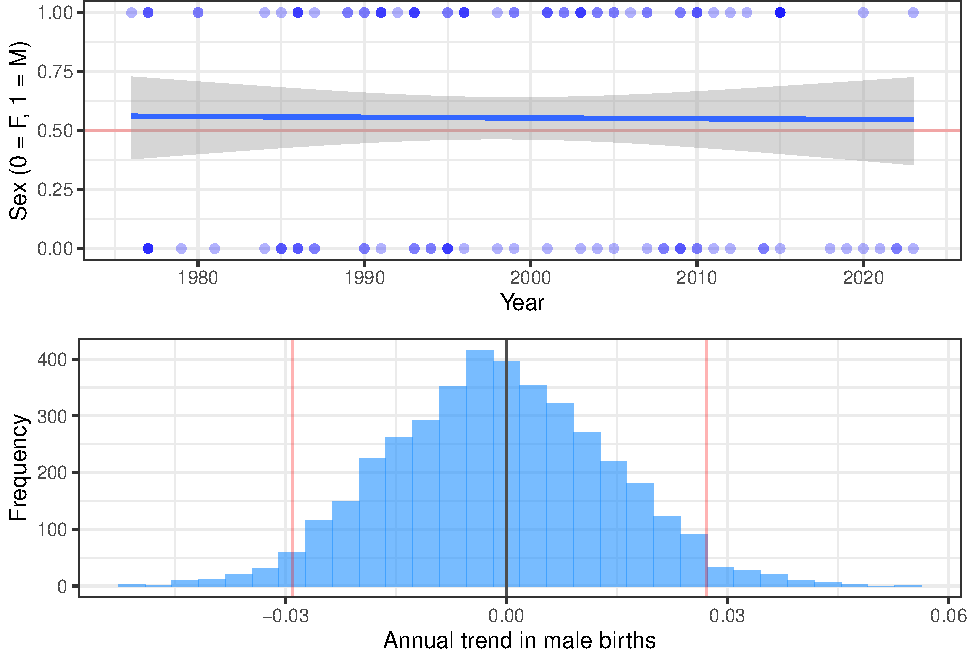
\includegraphics{status_update_files/figure-latex/unnamed-chunk-4-1.pdf}
\caption{Trends in sex ratio at births for Southern Resident killer
whales. Shown are all births (with GLM best fit) and the posterior
distribution of the coefficient for the year term (trend). Positive
values of the coefficient would support an increasing trend through
time. The red line on the top panel represents the 50:50 sex ratio, and
red lines on the histogram represent the 95\% CIs. \label{fig:srb}}
\end{figure}

\hypertarget{changing-population-structure}{%
\section{Changing Population
Structure}\label{changing-population-structure}}

One of the objectives of the recovery goals (NMFS 2008, 2011) was an age
and sex distribution that is more similar to the Northern Resident
population (at the time of ESA listing). The Southern Resident
population has undergone a number of shifts in age and sex, and because
the population is so small, the age or sex composition are more
sensitive to individual births and deaths. Previous status reviews based
these targets from 1973-1996 (Olesiuk, Ellis, and Ford 2005):

\begin{longtable}[]{@{}ll@{}}
\toprule
Stage &\tabularnewline
\midrule
\endhead
Juveniles & 47 \%\tabularnewline
Reproductive females & 24 \%\tabularnewline
Post-reproductive females & 11 \%\tabularnewline
Adult males & 18 \%\tabularnewline
\bottomrule
\end{longtable}

We can re-evaluate these targets, both for the Northern and Southern
Resident populations, using the most recent years of data available
(2018 for Northern Resident, 2021 for Southern Resident). There are some
small differences between life stages used in Olesiuk et al.~2005, and
more recent work (Ward et al. 2013). First, Olesiuk assumed animals to
not be mature to 15.5 (wheras Ward et al.~2013 assumed females to be
mature at age 10). Second, Olesiuk et al. (2005) defined
post-reproductive animals to be animals who hadn't given birth in 10
years (Ward et al.~2013 used a cutoff of 42 years). For these
calculations, we define age at maturity to be 10 years, and 42+ as the
age of reproductive senescence.

\begin{longtable}[]{@{}lllll@{}}
\toprule
& SRKW 1979 & SRKW 2021 & NRKW 1979 & NRKW 2018\tabularnewline
\midrule
\endhead
Juveniles (\textless{} 10) & 37 \% & 15 \% & 32 \% & 24
\%\tabularnewline
Adult males (10+) & 18 \% & 36 \% & 32 \% & 27 \%\tabularnewline
Adult females (10-42) & 27 \% & 38 \% & 31 \% & 40 \%\tabularnewline
Post-reproductive females (42+) & 19 \% & 11 \% & 4 \% & 8
\%\tabularnewline
\bottomrule
\end{longtable}

\hypertarget{reproductive-females}{%
\subsubsection{Reproductive females}\label{reproductive-females}}

The number of reproductive aged females was at its lowest point in the
late 1970s, in part because of the prior harvesting that occurred into
the early 1970s (Fig. \ref{fig:ts-repro-females}). Though the overall
number of reproductive females has been fluctuating between 25-35 for
most of the last 40 years, there have been contrasting changes by pod,
with declines in L pod females and increases in J pod (Fig.
\ref{fig:ts-repro-females}). At the start of the survey in 1976, the
distribution of females was skewed toward younger ages with few older,
post-reproductive females. The distribution in recent years is more
uniform across female ages (in other words, more females in their 30s,
Fig. \ref{fig:plot-repro-females}).

\begin{figure}
\centering
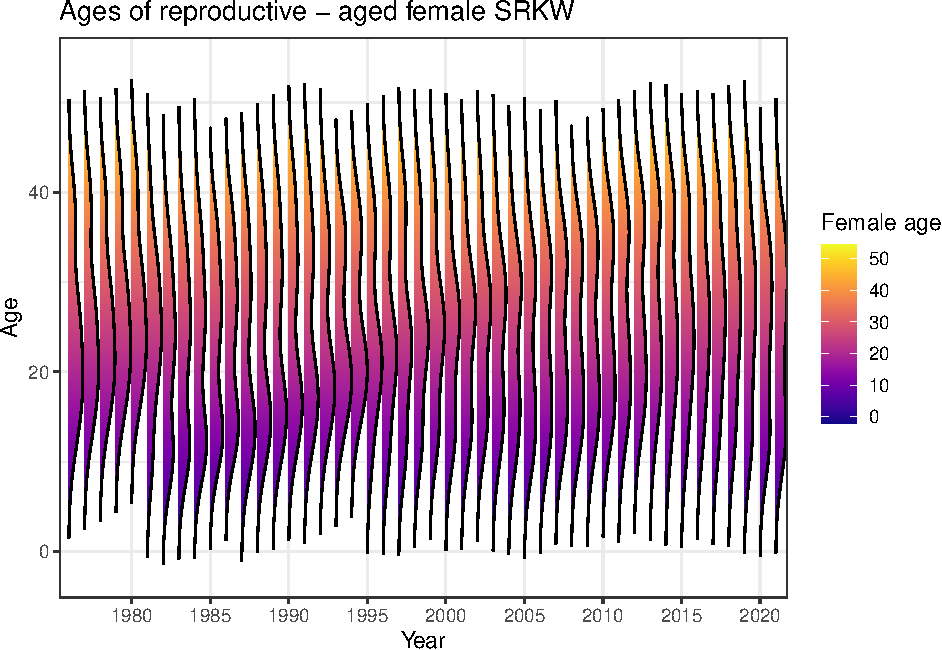
\includegraphics{status_update_files/figure-latex/reprofemales-1.pdf}
\caption{Distribution of ages of reproductive age females (10-42,
inclusive) for Southern Residents by year since 1976.
\label{fig:plot-repro-females}}
\end{figure}

\begin{figure}
\centering
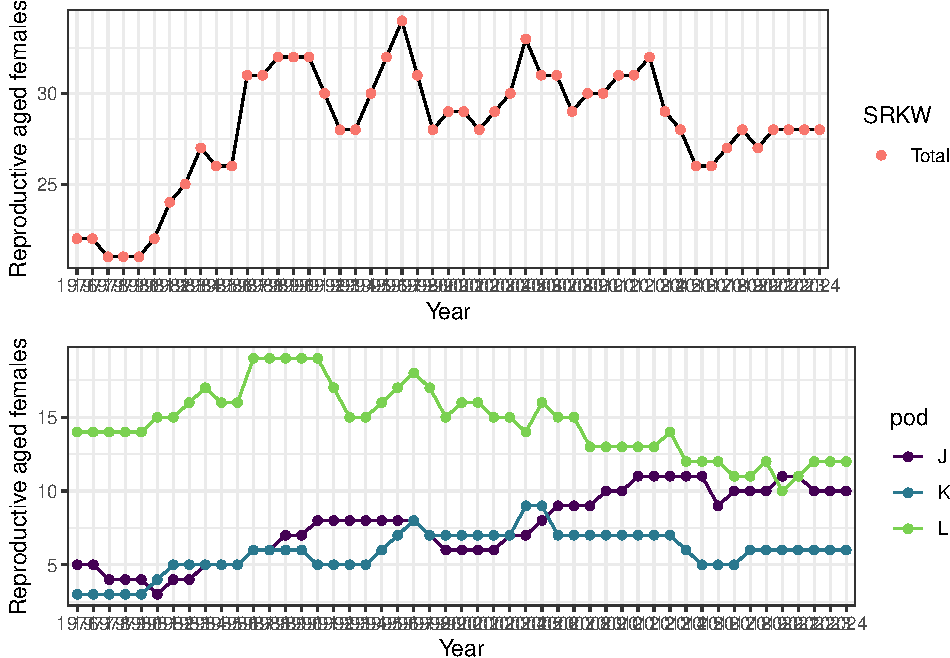
\includegraphics{status_update_files/figure-latex/reprots-1.pdf}
\caption{Time series of reproductive age females (10-42, inclusive) for
Southern Residents by year since 1976. \label{fig:ts-repro-females}}
\end{figure}

For comparison, we can also look at the aggregate number of reproductive
females in the NRKW population. This shows a nearly linear growth ovder
time (Fig. \ref{fig:ts-reprofemales-nr}).

\begin{figure}
\centering
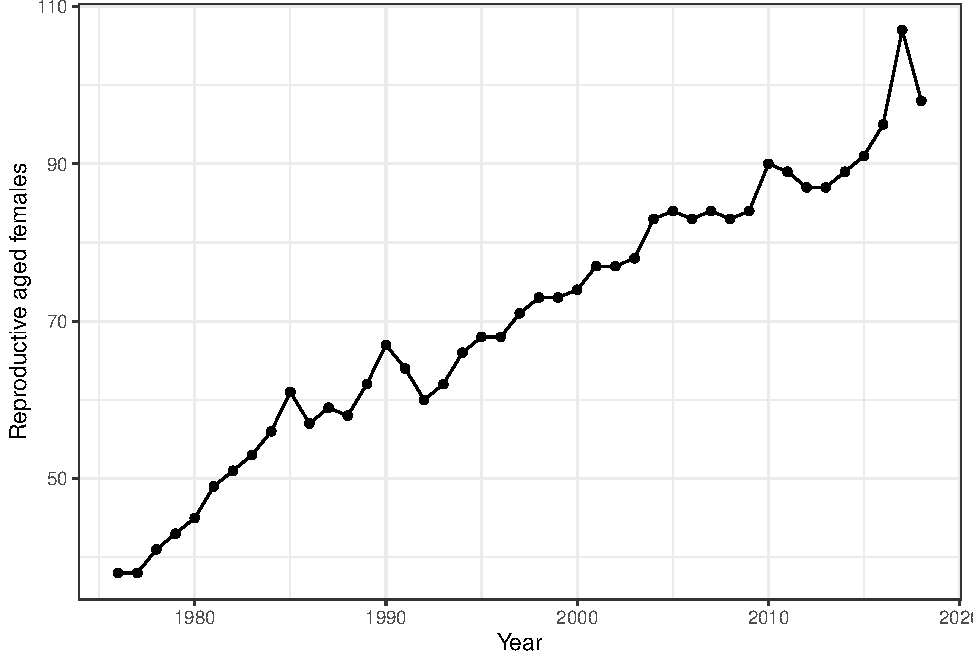
\includegraphics{status_update_files/figure-latex/reprots2-1.pdf}
\caption{Time series of reproductive age females (10-42, inclusive) for
Northern Residents by year since 1976. \label{fig:ts-reprofemales-nr}}
\end{figure}

\hypertarget{changing-demographic-rates}{%
\section{Changing demographic rates}\label{changing-demographic-rates}}

\hypertarget{increased-evidence-of-declining-fecundity}{%
\subsubsection{Increased evidence of declining
fecundity}\label{increased-evidence-of-declining-fecundity}}

There are several methodological changes from the projections done
previously (Hilborn et al. 2012; Ward et al. 2013). First, because we
don't indices of salmon abundance available to whales (and none of the
existing metrics of salmon abundance have been found to correlate with
killer whale demography; PFMC Draft Report 2019), the estimation model
was switched from a GLM to a GAM, which allows a smoother over year
effects. In terms of interpretation, these smooth terms represent annual
variation that may be driven by processes (prey, disease, etc) or
changes in data quality or detectability (particularly for birth rates,
which are partially a function of things like the fraction of time that
particular social groups spend in inland waters where they're more
likely to be seen). To evaluate changes in survival or fecundity rates
over time, we can examine survival rates estimated using data through
2010, versus estimates using data through 2021. For both instances, we
can fit generalized additive models (GAMs) that include the effect of
age (seperate splines by sex) and optionally a spline term over time. To
not introduce bias, we did not allow animals born \textless{} 1970 to be
included in the estimation (only the projection). For this sensitivity
analysis, the SRKW and NRKW data are combined into a single model, with
population as an estimated offset (Ward et al. 2013).

Results from these models indicate that of female survival, male
survival, and female fecundity, fecundity rates have changed the most
since 2010 and have declined (particularly for older ages, Fig.
\ref{fig:demo-rates}). Time series of estimated fecundity rates also
indicate low rates in recent years (this is not surprising, as there
have been very few successful births). Since 1980, there have been
several periods associated with high fecundity (late 1980s, mid 2000s,
Fig. \ref{fig:ts-demo}). In contrast, estimated survival rates have been
relatively flat (Fig. \ref{fig:ts-demo}), with the exception of low
survival prior to the population being listed (SRKW reached a peak of 98
animals in 1995, and then dropped to 82 animals in 2003).

\begin{figure}
\centering
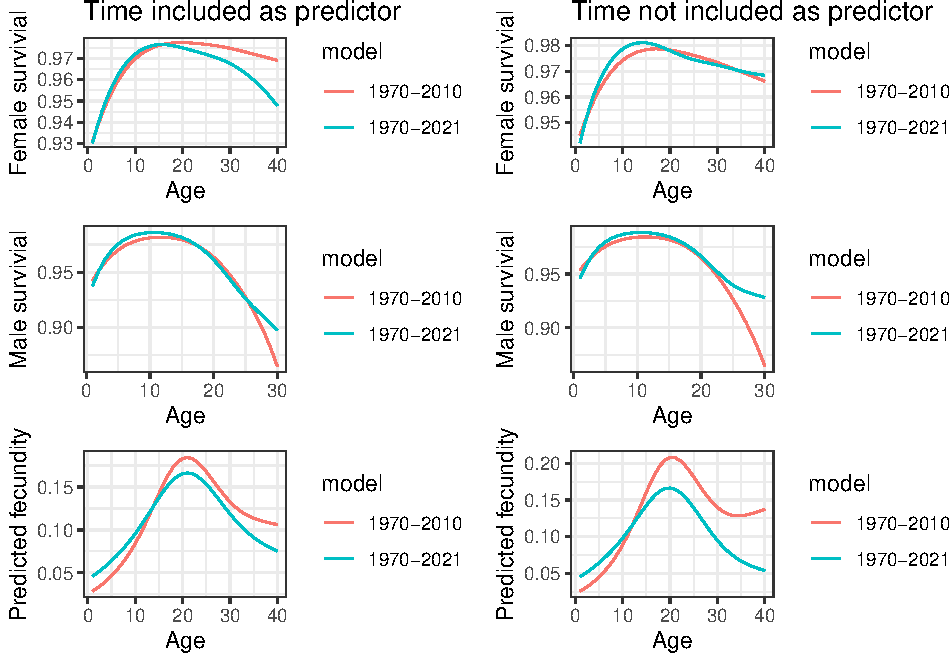
\includegraphics{status_update_files/figure-latex/unnamed-chunk-7-1.pdf}
\caption{Sensitivity analysis, showing how adding data since 2010
changes Southern Resident Killer whale demographic rates. Models with
time and age as predictors include smooth terms fit independently over
each predictor; models without time only include the age effect. All
models support the inclusion of year effects (not shown). Across rates,
these models illustrate little change in survival rates, and a decline
in fecundity rates since 2010. \label{fig:demo-rates}}
\end{figure}

\begin{verbatim}
#> [1] "projections/srkw_fec_age-year.rds"
\end{verbatim}

\begin{figure}
\centering
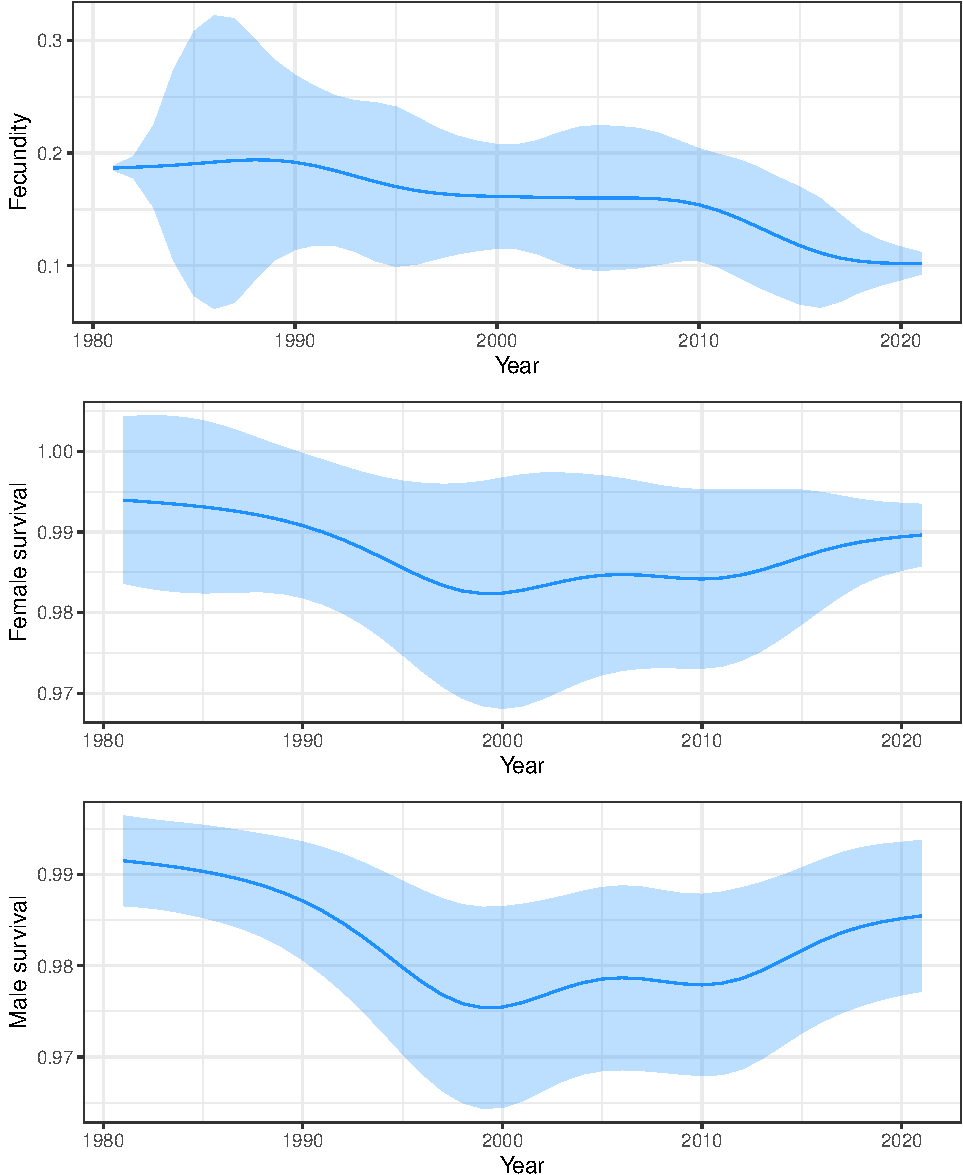
\includegraphics{status_update_files/figure-latex/figsurvrates-1.pdf}
\caption{Time series of predicted fecundity rates for a 20-year old
Southern Resident female killer whale and survival rates for a 20-year
old female and male. Estimates are generated from the Bayesian logistic
regression models, using priors from the NRKW population. Gray region
represents +/- 2 standard errors and the black line represents the mean.
\label{fig:ts-demo}}
\end{figure}

\break

\hypertarget{population-projections}{%
\section{Population projections}\label{population-projections}}

Given the current population age and sex structure, we performed a
series of forecasts or projections, doing 1000 simulations of 25 years
for each. Following previous work (Hilborn et al. 2012), projections
beyond this time frame were not included, as longer term trajectories
become negative, resulting in extinction or quasi-extinction. Following
previous annual updates, we also used a sex ratio at birth of 55\% male
/ 45\% female, because of the historical skew in SRKW sex ratios at
birth. Note that this differs from the previous reviews and published
projectsions, which assumes a 50:50 sex ratio at birth (Hilborn et al.
2012; Ward et al. 2013).

The scenarios we considered were:

\begin{enumerate}
\def\labelenumi{\arabic{enumi}.}
\tightlist
\item
  Projections using fecundity rates and survival rates estimated over
  the entire time series (this is done with estimation models ignoring
  time)\\
\item
  Projections using fecundity and survival rates estimated for the last
  5 years, 2016 to 2021\\
\item
  Projections using the highest fecundity and survival rates estimated,
  in the period 1985-1989
\end{enumerate}

\hypertarget{informative-priors}{%
\subsubsection{Informative priors}\label{informative-priors}}

Because this analysis was done in a Bayesian framework, we performed the
analysis with and without informative prior distributions (scenarios
without informative priors were based on Southern Resident data only).
Data provided by DFO have updated the NRKW catalog from 2010-2011 to
2018. As such, we can (1) consider informative priors on the effect of
age (for survival and fecundity rates), and (2) use informative priors
on the effect of year. We included scenarios with just informative
priors on age, or informative priors on the age and year terms (but not
informative priors on just year alone).

Fecundity was modeled using a Bayesian GAM (Wood 2016; Plummer 2019),
where

\[logit(p_{i,t})=B_{0} + f(year_{i,t}) + f(age_{i,t})\] where \(p_i\)
represents the probability of animal \(i\) giving birth at time \(t\),
\(B_{0}\) is a population specific intercept, and smooth functions
\(f()\) are modeled over year and age. As in GAMs fit with maximum
likelihood, the smooth functions can be written as
\(f(x)=\prod _{ j=1 }^{ J }{ { b }_{ j }{ z }_{ j }\left( x \right) }\),
where \(z_{j}\) are basis functions for the smoother, \(J\) is the
dimensionality, and \(b_{j}\) are estimated coefficients. Additional
details are provided in (Wood 2016).

Survival was also modeled using a logistic function, however we
implemented a stage- rather than age-based model, following limitations
of the data described in (Ward et al. 2013) and others. A primary
concern for example is that ages of older animals at the start of the
killer whale surveys were sometimes guessed based on reproductive
histories, and potentially biased. The survival model predicting
survival \(s_{i,t}\) of animal \(i\) at time \(t\) can be written as

\[logit(s_{i,t})=B_{0} + B_{stage} + f(year_{i,t})\] where \(B_{0}\) is
the population level offset, \(B_{stage}\) is a stage-specific effect
(stages as described in (Ward et al. 2013)) and \(f(year_{i,t})\) the
smooth term over years.

The fecundity and survival models were first fit to the NRKW data, using
weakly informative priors, 50000 Markov chain Monte Carlo (MCMC)
iterations, and 3 parallel MCMC chains. Output from the posterior
distributions of these models were used to generate multivariate normal
prior distributions for the SRKW population models. The effects of age
or stage and year were separated, and the posterior mean and
variance-covariance matrix of each was summarized.

Projections done for the 2016 Status Review (NMFS 2016) also showed the
population on a downward trajectory, and all three scenarios presented
here provide further evidence of a declining population over the next 25
years (Fig. \ref{fig:proj1}). The most optimistic scenario, using
demographic rates calculated from the 1985-1989 period, has a trajectory
that increases and eventually declines after 2030. Additional runs for
this scenario indicated a similar trajectory with a 50:50 sex ratio.
Thus, this downward trend is likely driven by the current age and sex
structure of young animals in the population, as well as the number of
older animals. For example, there's currently 0 females younger than 25
-- if all survive another 10 years, they will represent the majority of
the reproductive females in the population and number fewer than the
current population of reproductive females \ref{fig:plot-repro-females}.

A first set of projections represents the SRKW population projected
using the NRKW age/stage priors, but not including priors on the year
terms (essentially letting each population have different patterns over
time). This

\begin{figure}
\centering
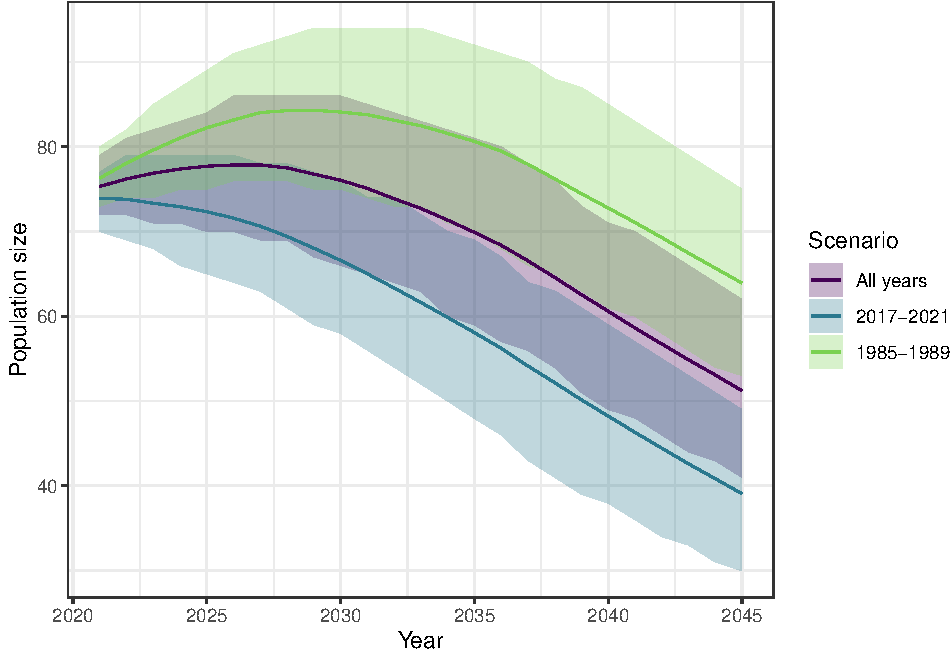
\includegraphics{status_update_files/figure-latex/proj1-1.pdf}
\caption{25-year projections of the SRKW population, using the NRKW age
and stage data as prior distributions for the SRKW parameters, but not
including priors on the year effects estimated from the NRKW population
\label{fig:proj1}}
\end{figure}

The sensitivity comparing the SRKW projections under different prior
distributions illustrated that for most scenarios, there appeared to be
little effect of using the prior on year effects, in addition to age.
Perhaps the scenario that showed the largest effect was the most
optimistic scenario, using survival and birth rates from the 1985-1989
period (Fig. \ref{fig:proj2}).

\begin{figure}
\centering
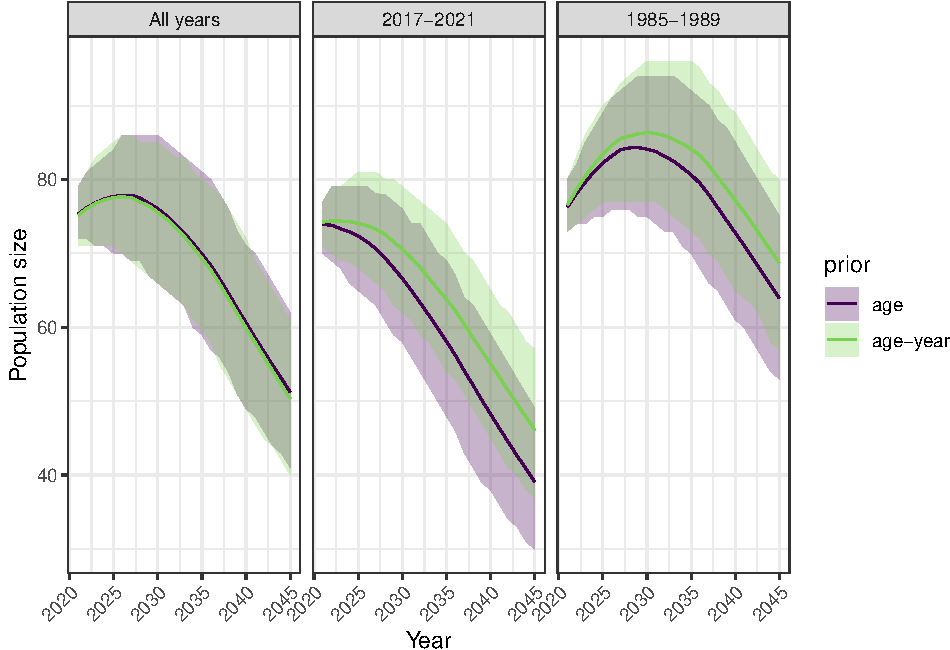
\includegraphics{status_update_files/figure-latex/proj2-1.pdf}
\caption{25-year projections of the SRKW population, using the NRKW age
/ stage and year prior distributions for the SRKW parameters, estimated
from the NRKW population \label{fig:proj2}}
\end{figure}

It's also important to understand future changes to reproductive SRKW
females (age 10-43). These plots use the same data as the projections
for the whole population. The uncertainty bands around the projections
are tightest for the next 10 years (those are based on animals currently
alive in the population) -- but uncertainty increases in the future, as
new simulated animals are added (Fig. \ref{fig:proj3}).

\begin{figure}
\centering
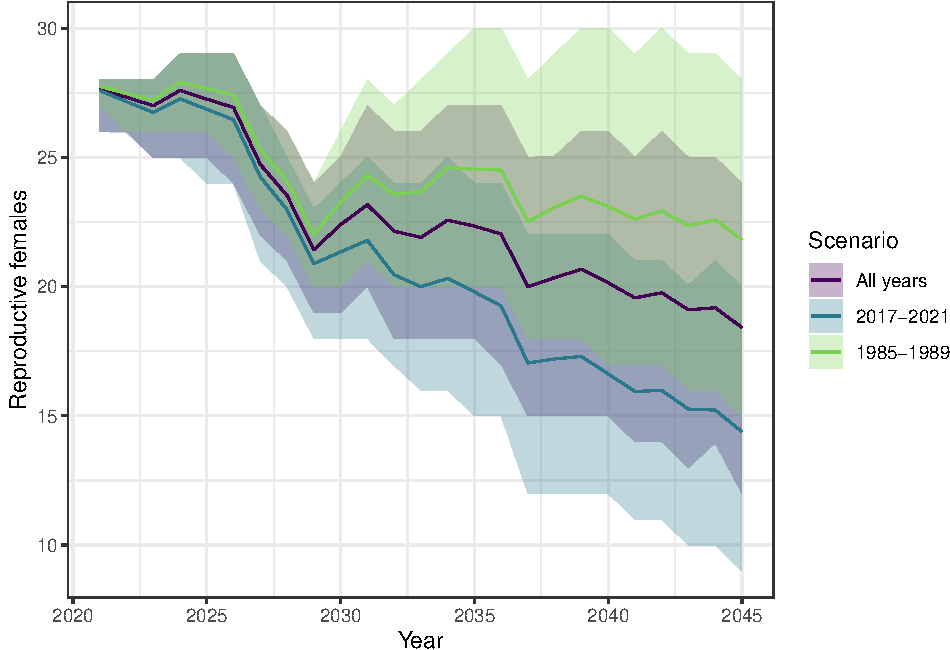
\includegraphics{status_update_files/figure-latex/proj3-1.pdf}
\caption{25-year projections of SRKW reproductive females (10-43), using
the NRKW age and stage data as prior distributions for the SRKW
parameters, but not including priors on the year effects estimated from
the NRKW population \label{fig:proj3}}
\end{figure}

\hypertarget{variation-in-individual-reproductive-success}{%
\subsubsection{Variation in individual reproductive
success}\label{variation-in-individual-reproductive-success}}

One of the factors that may contribute to SRKW declining faster than
these projections represent is individual variation in reproductive
success. All of the current modeling efforts assume that every female
has the same probabilities of giving birth (adjusted for age and year).
From an estimation standpoint, it's very difficult to fit more complex
models that let individuals have unique rates, when reproductive
histories are only partially observed. These generally result in
estimates for young animals with wide confidence intervals.

But we can look at the current potential moms in the population, and
identify ones that haven't reproduced in the last decade. While there
are 26 potential moms, 9 haven't given birth in the last decade, because
of age or other reasons. Looking forward a decade and filtering these
and older animals out, if the remaining all live there will be 16. Of
the living SRKW animals who aren't yet of reproductive age, there are 4
confirmed females and 2 of unknown sex -- so if all these animals
survive and are female, we'd expect to have 22 SRKW moms in 10 years.

\begin{longtable}[]{@{}lrrl@{}}
\toprule
animal & age & last\_birth & unlikely\_future\_mom\tabularnewline
\midrule
\endhead
J019 & 42 & 2005 & *\tabularnewline
J022 & 36 & 2003 & *\tabularnewline
J031 & 26 & 2019 &\tabularnewline
J036 & 22 & 2015 &\tabularnewline
J037 & 20 & 2015 &\tabularnewline
J040 & 17 & NA &\tabularnewline
J042 & 14 & NA &\tabularnewline
J046 & 12 & NA &\tabularnewline
J047 & 11 & NA &\tabularnewline
K016 & 36 & 2002 & *\tabularnewline
K020 & 35 & 2004 & *\tabularnewline
K022 & 34 & 2006 & *\tabularnewline
K027 & 27 & 2011 & *\tabularnewline
K042 & 13 & NA &\tabularnewline
K043 & 11 & NA &\tabularnewline
L072 & 35 & 2005 & *\tabularnewline
L077 & 34 & 2019 &\tabularnewline
L082 & 31 & 2010 & *\tabularnewline
L083 & 31 & 2007 & *\tabularnewline
L086 & 30 & 2014 &\tabularnewline
L090 & 28 & NA &\tabularnewline
L091 & 26 & 2015 &\tabularnewline
L094 & 26 & 2015 &\tabularnewline
L103 & 18 & 2015 &\tabularnewline
L113 & 12 & NA &\tabularnewline
L118 & 10 & NA &\tabularnewline
\bottomrule
\end{longtable}

\break

\hypertarget{acknowledgments}{%
\section{Acknowledgments}\label{acknowledgments}}

Annual data for SRKW was collected by the Center for Whale Research.
Recent updates to the NRKW catalog (initially provided by John Ford in
2011) and help interpreting data were provided by Thomas Doniol-Valcroze
and Jared Towers.

\hypertarget{references}{%
\section*{References}\label{references}}
\addcontentsline{toc}{section}{References}

\hypertarget{refs}{}
\leavevmode\hypertarget{ref-hilborn2012}{}%
Hilborn, R., Cox S.P., Gulland F.M.D., Hankin D.G., Hobbs N.T., and D.E.
Schindler. 2012. ``The Effects of Salmon Fisheries on Southern Resident
Killer Whales: Final Report of the Independent Science Panel.'' ESSA
Technologies Ltd., Vancouver, B.C.

\leavevmode\hypertarget{ref-nmfs2008}{}%
NMFS. 2008. ``Recovery Plan for Southern Resident Killer Whales (Orcinus
Orca).'' National Marine Fisheries Service, Seattle, WA.

\leavevmode\hypertarget{ref-nmfs2011}{}%
---------. 2011. ``Southern Resident Killer Whales (Orcinus Orca) - 5
Year Review: Summary and Evaluation.'' National Marine Fisheries
Service, Seattle, WA.

\leavevmode\hypertarget{ref-nmfs2016}{}%
---------. 2016. ``Southern Resident Killer Whales (Orcinus Orca) - 5
Year Review: Summary and Evaluation.'' National Marine Fisheries
Service, Seattle, WA.

\leavevmode\hypertarget{ref-olesiuk2005}{}%
Olesiuk, Peter, Graeme M. Ellis, and John K.B. Ford. 2005. ``Life
History and Population Dynamics of Northern Resident Killer Whales
(Orcinus Orca) in British Columbia.'' CSAS 2005/045. Fisheries and
Oceans Canada. \url{https://doi.org/10.3386/w11467}.

\leavevmode\hypertarget{ref-pfmc2020b}{}%
PFMC. 2020a. ``Pacific Fishery Management Council Salmon Fishery
Management Plan Impacts to Southern Resident Killer Whales: Draft Range
of Alternatives and Recommendations.''
\url{https://www.pcouncil.org/documents/2020/08/h-3-a-srkw-workgroup-report-1-pacific-fishery-management-council-salmon-fishery-management-plan-impacts-to-southern-resident-killer-whales-draft-range-of-alternatives-and-recommendations.pdf/}.

\leavevmode\hypertarget{ref-pfmc2020}{}%
---------. 2020b. ``Pacific Fishery Management Council Salmon Fishery
Management Plan Impacts to Southern Resident Killer Whales: Risk
Assessment.''
\url{https://www.pcouncil.org/documents/2020/02/e-3-a-srkw-workgroup-report-1-electronic-only.pdf/}.

\leavevmode\hypertarget{ref-plummer2019}{}%
Plummer, Martyn. 2019. \emph{Rjags: Bayesian Graphical Models Using
Mcmc}. \url{https://CRAN.R-project.org/package=rjags}.

\leavevmode\hypertarget{ref-ward2013}{}%
Ward, Eric J., Mike J. Ford, R.G. Kope, Ford J.K.B., A. Velez-Espino,
C.K. Parken, L. LaVoy, M.B. Hanson, and K.C. Balcomb. 2013. ``Estimating
the Impacts of Chinook Salmon Abundance and Prey Removal by Ocean
Fishing on Southern Resident Killer Whale Population Dynamics.''
NMFS-NWFSC-123. U.S. Department of Commerce, NOAA.

\leavevmode\hypertarget{ref-wood2016}{}%
Wood, S. 2016. ``Just Another Gibbs Additive Modeller: Interfacing Jags
and Mgcv.'' \url{https://arxiv.org/pdf/1602.02539.pdf}.

\end{document}
